\documentclass[12pt]{article}
	
	%%%%%%%%%%%%%%%%%%%%%%%%%%%%%%%%%%%%%%%%%%%%%%%%%%%%%%%%%%%%%%%%%%%%%%
	%\pdfminorversion=4
	% NOTE: To produce blinded version, replace "0" with "1" below.
	\newcommand{\blind}{0}
	
	%%%%%%% IISE Transactions margin specifications %%%%%%%%%%%%%%%%%%%
	% DON'T change margins - should be 1 inch all around.
	\addtolength{\oddsidemargin}{-.5in}%
	\addtolength{\evensidemargin}{-.5in}%
	\addtolength{\textwidth}{1in}%
	\addtolength{\textheight}{1.3in}%
	\addtolength{\topmargin}{-.8in}%
    \makeatletter
    \renewcommand\section{\@startsection {section}{1}{\z@}%
                                       {-3.5ex \@plus -1ex \@minus -.2ex}%
                                       {2.3ex \@plus.2ex}%
                                       {\normalfont\fontfamily{phv}\fontsize{16}{19}\bfseries}}
    \renewcommand\subsection{\@startsection{subsection}{2}{\z@}%
                                         {-3.25ex\@plus -1ex \@minus -.2ex}%
                                         {1.5ex \@plus .2ex}%
                                         {\normalfont\fontfamily{phv}\fontsize{14}{17}\bfseries}}
    \renewcommand\subsubsection{\@startsection{subsubsection}{3}{\z@}%
                                        {-3.25ex\@plus -1ex \@minus -.2ex}%
                                         {1.5ex \@plus .2ex}%
                                         {\normalfont\normalsize\fontfamily{phv}\fontsize{14}{17}\selectfont}}
    \makeatother
    %%%%%%%%%%%%%%%%%%%%%%%%%%%%%%%%%%%%%%%%%%%%%%%%%%%%%%%%%%%%%%%%%%%%%%%%%
	
	%%%%% IISE Transactions package list %%%%%%%%%%%%%%%%%%%%%%%%%%%%%%%%%%%%%%
	\usepackage{amsmath}
	\usepackage{graphicx}
	\usepackage{enumerate}
	\usepackage{natbib} %comment out if you do not have the package
	\usepackage{url} % not crucial - just used below for the URL
	\usepackage{hyperref}
	%%%%%%%%%%%%%%%%%%%%%%%%%%%%%%%%%%%%%%%%%%%%%%%%%%%%%%%%%%%%%%%%%%%%%%%
	
	%%%%% Author package list and commands %%%%%%%%%%%%%%%%%%%%%%%%%%%%%%%%%%%%%%%%%%%%%
	%%%%% Here are some examples %%%%%%%%%%%%%%
	%	\usepackage{amsfonts, amsthm, latexsym, amssymb}
	%	\usepackage{lineno}
	%	\newcommand{\mb}{\mathbf}
	%%%%%%%%%%%%%%%%%%%%%%%%%%%%%%%%%%%%%%%%%%%%%%%%%%%%%%%%%%%%%%%%%%%%%%%%%%%%%%
	
	
	\begin{document}
		
			%%%%%%%%%%%%%%%%%%%%%%%%%%%%%%%%%%%%%%%%%%%%%%%%%%%%%%%%%%%%%%%%%%%%%%%%%%%%%%
		\def\spacingset#1{\renewcommand{\baselinestretch}%
			{#1}\small\normalsize} \spacingset{1}
		%%%%%%%%%%%%%%%%%%%%%%%%%%%%%%%%%%%%%%%%%%%%%%%%%%%%%%%%%%%%%%%%%%%%%%%%%%%%%%
		
		\if0\blind
		{
			\title{\bf Agricultural Dependence in Mexico}
			
			\author{ William Townsend  \\
			Department of Economics, The University of Oklahoma, Norman\\
             }
			\date{\today}
			\maketitle
		} \fi
		
		\if1\blind
		{

            \title{\bf \emph{} \LaTeX \ Template}
			\author{Author information is purposely removed for double-blind review}
			
\bigskip
			\bigskip
			\bigskip
			\begin{center}
				{\LARGE\bf \emph{IISE Transactions} \LaTeX \ Template}
			\end{center}
			\medskip
		} \fi
		\bigskip
		
%		
%	\begin{abstract}
%This document provides a \LaTeX \ template for \emph{IISE Transactions}. Your paper should be compiled in the following order: title; abstract; keywords; main text, including an introduction and a conclusion or summary; acknowledgments; declaration of interest statement; references; appendices (as appropriate). Figures and tables should be inserted into the text as close to first mention as possible (NOT appended to the end of the manuscript). In-text citations and the reference list must follow \emph{IISE Transactions} guidelines. Use 11 point font, 1 inch margins, and double-spacing for the manuscript. A typical paper for this journal should be no more than 30 pages in manuscript format, counting from the title page to references. Appendices should be included as supplemental online materials. Do not use footnotes. \emph{IISE Transactions} uses a double-blind review process. Please make sure that you submit the \textbf{blind version} of your manuscript, which does not contain any information identifying the authors.  This includes removing the authors information on the title page as well as the information that may be identifying in the Acknowledgment section. We thank you for your attention to these details.
%	\end{abstract}
%			
%	\noindent%
%	{\it Keywords:} \emph{IISE Transactions}; \LaTeX; Manuscript format; Taylor \& Francis.
%
%	%\newpage
%	\spacingset{1.5} % DON'T change the spacing!

\section{Abstract} \label{s:intro}

Standard Ricardian trade theory suggests that countries should prioritize production in goods where they have a comparative advantage. A growing body of literature suggests that Ricardo's work should be taken with a grain of salt. Countries who prematurely open their economy to the international market and do not properly develop their manufacturing sector grow more slowly. A lack of manufacturing diversification tends to come from an economy becoming overly dependent in its agricultural sector. Thus, an over dependence of agricultural production can lead to worse economic conditions within a country. Much of Latin America suffers from slow economic growth due to premature trade openness and over dependence in its agricultural sector. Latin America has also faced abnormally high homicide rates, especially in countries such as Mexico. In this paper, I hypothesize that a greater dependence of agricultural sales leads to higher homicide rates in Mexico. I test this hypothesis using OLS and 2SLS measures. While some trends show that dependence of international agricultural sales is correlated with higher homicide rates in Mexico, the empirical results are not consistent. Thus, based on this paper's empirical work, one cannot conclude whether higher agricultural dependence causes higher homicide rates in Mexico.  
\newpage
\section{Introduction} \label{s:sec2}

\begin{itemize}
  \item Mexico's homicide rates have dramatically increased from 2010 to 2020. For example, Mexico's Secretariat of Security and Citizen Protection and Executive Secretary of the National Public Security System of Government show disturbing spike's of homicide at the state level. Their data shows that in the state of Baja California the homicide rate per 100,000 residents increased from 27.41 in 2010 to 70.15 in 2020. In Michoacan, the homicide rate increased from 14.95 to 43.65 in 2010 and 2020, respectively.  Colima went from a homicide rate of 14.11 to 71.08 in 2010 and 2020 respectively.  
  \item Mexico's Security, Justice and Peace department announced that in 2020 that the five most violent cities in the world were all in Mexico. These cities are Tijuana, Juarez, Uruapan, Irapuato, and Ciudad Obregon.
  \item There is growing literature and knowledge of a strong relationship between Mexico's drug cartels and their agricultural sector. For example, \cite{O'Dowd} from WBUR reported in 2020 how there was growing evidence showing the involvement of Mexican cartels in the avocado industry. In February 2020, Mexican officials found the body of a second murdered activist. The murdered activist worked at the Monarch Butterfly Biosphere Reserve in the mountains of Michoacán. Reports on the case stated the murders had something to do with clandestine avocado farms. Unfortunately, Mexican drug cartels found a way to break into the rapidly growing and profitable avocado business in Michoacán. Michoacán is the state that exports most of the Mexico's avocados. Eduardo Moncada, an assistant political science professor at Barnard College stated in the WBUR report that cartels have been diversifying their portfolios to have a wider range of legal economies in addition to drugs and trafficking. In the state of Michoacán, avocados are a major source of income. Thus, cartels have been capturing money from that sector. Cartels accomplish this through extortion of avocado producers, transporters, and packers. They also take over lands used to produce avocados. In doing so, they become informal owners of the avocado orchards. Cartels have broadened their horizon to also control other agricultural goods such as wood and timber. Avocado farmers initially welcomed cartels into their businesses because they offered security for themselves, their land, and products. These were services that the government could not provide. Cartels charged a tax for their service but became more predatory over time. ``Cartels stopped providing the growers with services but kept charging extortion fees", \cite{O'Dowd}.
  \item The major focus of this paper will be to draw the connection between Mexico's dependence on its agricultural sector impacting crime. More specifically, I will assess whether higher dependence of of agricultural sales over total sales on the international market causes higher crime. In section 3, I will go over a literature of this topic.  Section 4 will include my data sources and empirical strategy. Section 5 will discuss the analysis's results and in section six I will make concluding remarks.
\end{itemize} 



\section{Literature Review}\label{s:sec3}

\begin{itemize}
    \item \cite{beittel2015mexico} discusses the history and development of Mexico's major drug trafficking cartels (DTOs). This paper is important for developing my cartel dummy variable that I will discuss in the next section.
    \item \cite{erickson2020blood} assess whether growing demand for licit goods is causing increased violence among Mexican criminal organizations. When running a difference-in-differences model, they discover that in Michoacán and Jalisco there was a decrease in homicide after the Mexican Hass Avocado Import Program of 2016. The policy lifted Mexico avocado import restrictions. The paper concluded that an increased demand of avocado lead to a decrease in homicide. This paper also discusses in great detail how farmers pay protection fees to drug cartels.
    \item \cite{dube2016maize} show that when maize prices increase, farmers are more likely to produce more corn to reap higher profits. However, when maize prices drop, farmers tend to grow more illicit crops such as Marijuana and poppy. This phenomena shows that farmers have an economic incentive to produce more licit goods when positive shocks, like maize price increases, take place.
    \item \cite{leenen2014temporal} discovered, through logistic modeling, that the highest homicide rates occurred in areas with the highest drug trafficking.They discovered, through logistic modeling, that the highest homicide rates occurred in areas with the highest drug trafficking. In addition, more densely populated areas experienced higher intentional murder rates. In other words, homicides are more common among urban areas than sparsely populated regions.
    \item \cite{gamlin2015violence} discusses a multivariate analysis done by researchers at Guadalajara University. Their findings concluded that lawlessness, drug trafficking, alcohol or drug consumption, and basic education dropout were key causal determinants of increased homicide rates in Mexico.
    \item \cite{lopez2014narcotrafico} add to the literature, stating poverty and economic inequality are the causal factors of murder rates, not lawlessness. Regardless of conflicting views of causality, an agreed upon concept is the Mexican Government appears to not be able to guarantee the safety of its citizens.
    \item \cite{briceno2008understanding} argue that higher homicide rates in Latin American countries stems from nations' social contexts and political models. The social contexts they refer to are income inequality and labor wages. Poverty and youth unemployment can also lead to the loss of mechanisms of social control, such as family and religion. The authors conclude that four major factors increase violence: the specific structure of the built environment in cities, the culture of masculinity, drug market presence, and ineffective judicial systems. 
    \item Economic analysis has begun to evaluate the impact global trade has on Mexico's crime rate. \cite{dell2019violent} claim that loss of manufacturing jobs from competition with China increased cocaine trafficking and violence. When Mexican laborers become more desperate in finding ways to make enough money, they often have little to no other choices for work outside criminal employment. The evidence presented in their paper supports a Becker-style model where elasticity between criminal and legitimate employment is extremely high. Specifically, this high elasticity takes place in locations where criminal organizations lower illicit job search costs, where the drug trade implies greater pecuniary returns to violent crime, and lastly where unemployment dis-proportionally impacts low-skilled men more than high-skilled men. When drug transportation becomes more lucrative and low skill workers have less opportunity cost in joining criminal employment, more people get involved in illegal activity. These authors conclude that the Mexican government should focus on social safety and strengthening the manufacturing sector. The study from \cite{dell2019violent} shows the need to maintain a strong manufacturing sector. It also presents a danger from freer trade when a country, such as Mexico, cannot compete on the international market. Industrial protection in certain manufacturing sectors could be critical for Mexico to mitigate its violent crimes. While there are many benefits to more open trade, Mexico appears to have  prematurely open itself up too freely.
    \item \cite{dell2015trafficking} uses regression discontinuity to show how close elections of PAN mayors in Mexico lead to higher homicide rates in municipalities. Cracking down on cartel crime is among the PAN party's top priorities. Thus, when PAN mayors come into off after a close election, cartels lash out to maintain their territory. Ultimately these cartels end up migrating to a different municipality. 
\end{itemize}

\newpage

\section{Empirical Work and Modeling} \label{s:sec4}
\begin{itemize}
    \item In order to run empirical work on this topic, I collected and arranged my own unique data set from multiple government sources. This paper evaluates data at the Mexican state level on an annual basis. The data extends 11 years from 2010 to 2020. My variable in question is Sales. I calculate this variables in the following way:
    
    $$Sales=\frac{Agriculture}{Total}$$
    
    Agriculture stands for the total crops sold at the international level. The denominator is the total international sales each state has in a given year. Data for this variable comes from the Secretaría de Economía.
    
    \item My dependent variable is logged homicide rates per 100,000 residents. To collect this data, I scraped a wikipedia page that displayed the homicide rates of all 32 states from 2006 to 2020. I double checked the validity of the data and found that the homicide rates come from The Secretariat of Security and Citizen Protection and Executive Secretary of the National Public Security System of Government. I also found that this data matched records in Mexico's National Institute of Statistics and Geographics (INEGI). The next three images display images I created in Rstudio. I will clean these images up in my final draft. 
    
    \item The first image shows the spread of homicide in each state in each year over the years 2010 to 2020. The blue line sadly indicates a gradual increase of homicide among the country.
    
    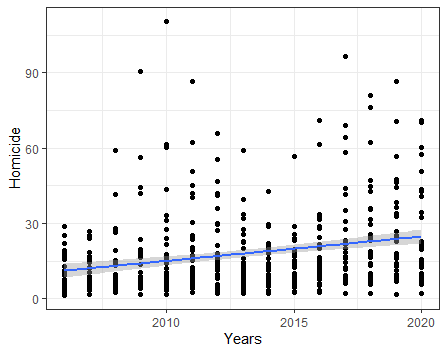
\includegraphics[]{PS6a_Townsend.png}
    
    \item This image shows the distribution of the homicide rates from 2006 to 2020.
    
    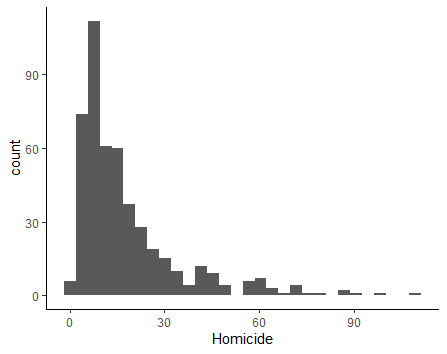
\includegraphics[]{PS6b_Townsend.png}
    
    \item In this last image I have logged homicide rates to normalize the variable. This method will help make interpreting the coefficients more simple with percentages.
    
    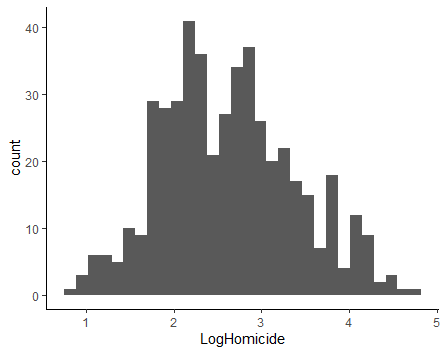
\includegraphics[]{PS6c_Townsend.png}
    
    \item
    My model also includes the dummy variables cartel and border. The dummy border has a value of 1 when a state borders the U.S. Its value is 0 otherwise. Cartel equals 1 when a state hosts a major cartel organization. Its value is 0 otherwise. This dummy was constructed through information in \cite{beittel2015mexico}.
    
    \item Table 1 is far from complete. This is truly only a rough draft and only showing what direction I'm going. I have data for more independent variables such as unemployment rates from Encuesta Nacional de Ocupacion y Empleo (ENOE) and average state temperatures from the World Bank. I will also lag the log homicide rates and treat that as another independent variables. Lastly, I will use average precipitation each year as an instrumental variable on my Sales variable. This data also comes from the World Bank.
    
    \item My final model will apply both OLS and 2SLS. I will also run a variety of regressions testing what happens when I have no fixed effects, year fixed effects, state fixed effects, and both year and state fixed effects. 
    
    \item I firmly believe there is a strong argument for using average annual precipitation as an IV for my sales variable. It would be very hard to argue that precipitation directly impacts homicide rates. In addition, it would also be hard to argue that precipitation would most likely be correlated with anything else in the error term of the model. However, precipitation does greatly impact agricultural production. My only hesitancy would be that precipitation is correlated with temperature, which I intend to use as an independent variable. Not that I believe much correlation is happening between precipitation to temperature to finally homicide rates, but this is still a possibility. Thus, I'm not saying the IV is 100 percent perfect, but I argue it is still very good. 
    
    \item Table one is a premature table showing some of my results. My total analysis includes 352 observations. 
    
    \item For now, my empirical modeling for year and state fixed effects is the following where Y is logged homicide. Both i and t stand for states and years, respectively. Sales is the coefficient of interest, X is my vector of controls, S is my state fixed effects, T is year fixed effects, and $\varepsilon$ is the error term: 
    

    \item The following represents the two-way fixed effect model for both states and years.  
    
    $$Y_{it}=\alpha+\beta_1Sales\beta_2 X_{it}+S_i+T_t+\varepsilon_{it}$$
$$i\in \{1,2,...,22\}$$
$$t \in \{2012, 2013,...,2020\}$$

\item My final draft will have a more complete set up of both my first stage and second stage equations for the incorporation of my precipitation IV.
    
    
\end{itemize}


%%%%%%%%%%%%%%%%%%%
%% Regression TABLE
%%%%%%%%%%%%%%%%%%
\FloatBarrier
\begin{table}[h]
  \begin{threeparttable}
 
  \caption{Empirical Results}\centering
  \small
\begin{tabular}{lllll}
\hline \hline 
\cline { 2 - 7 } & \multicolumn{4}{c}{Logged Homicide Rates} \\
\hline & $(1)$ & $(2)$ & $(3)$ & $(4)$ \\
\hline Border & $0.507^{***}$ & $0.503^{***}$ & $1.317^{***}$ & $1.354^{***}$  \\
& $(0.0850)$ & $(0.0862)$ & $(0.191)$ & $(0.151)$  \\
Cartel & $0.558^{***}$ & $0.560^{***}$ & $0.170$ & $0.127$  \\
& $(0.0780)$ & $(0.0766)$ & $(0.143)$ & $(0.103)$  \\
Agriculture Sales & $0.775^{***}$ & $0.758^{***}$ & $0.485$ & $0.241$ \\
& $(0.142)$ & $(0.138)$ & $(0.241)$ & $(0.230)$ \\


Constant & $29.622^{* * *}$ & $12.502^{* * *}$ & $30.935$ & $19.353$ \\
& $(6.096)$ & $(4.694)$ & $(20.687)$ & $(14.468)$ \\

\hline Observations & 352 & 352 & 352&352 \\
Adjusted R^2 & 0.236 & 0.286 & 0.737 & 0.789  \\
Year FE & No & Yes & No & Yes  \\
State FE & No & No & Yes & Yes  \\
%Non selected & 206 & 186 & 166 & 154 & 150 & 144 \\
\hline \hline
\end{tabular}
   \begin{tablenotes}\left
      \scriptsize
      
\textit{Note:} In (1), I run a standard OLS with no fixed effects. Column (2) includes an OLS regression with only year fixed effects. Column (3) is a regression with state fixed effects. Lastly, (4) is an OLS with both year and state fixed effects.    $* p<0.1 ; * * p<0.05 ; * * * p<0.01$
    \end{tablenotes}
  \end{threeparttable}
\end{table}
\FloatBarrier
%%%%%%%%%%%%%%%%%%%%%%%%%%%%%%%%%%%%%%

\newpage

\section{Discussion} \label{s:sec5}

\begin{itemize}
    \item So far my table consistently shows strong statistically significant results for my border dummy. This is not a surprise. I do not expect this result to change for my final draft because a lot of drug trafficking takes place at the U.S. and Mexico border. My cartel dummy is only statistically significant for my first two columns. When I have either state fixed effects or both state and year fixed effects, it is no longer statistically significant. The same is true for my Sales variable. My $R^2$ has good values ranging from 0.236 to 0.789. 
    \item I expect my results to change once I include lagged homicide, unemployment, average temperatures, and my precipitation instrumental variable.
    \item What are your thoughts on me running state fixed effects and or running two-way state and year fixed effects? I believe my results are showing to be unsteady due to a lack of variation. I only have 11 years, thus I don't know if I should only include year fixed effects. My feeling is that agricultural ratios within a single state for 32 states will not dramatically change over solely 11 years.
    
\end{itemize}

\newpage

\section{Conclusion} \label{s:sec6}

\begin{itemize}
    \item So far my empirical analysis needs to include more variables. As of now the empirical work suffers from severe omitted variable bias. In addition, I need to run the precipitation IV to see how endogeneity of my Sales variable potentially impacts the OLS results.  
\end{itemize}







 
 
 




%\if0\blind{
%\section*{Acknowledgements}
%The authors acknowledge the generous support from the funding agency of XYZ.	} \fi
\newpage
\bibliographystyle{chicago}
\spacingset{1}
\bibliography{Trans}

\newpage
\cite{Security}
\cite{Secretariat97-17}
\cite{Seguridad}
\cite{Seguridad2018}
\cite{Seguridad2020}
\cite{Economia}
\cite{Wage}
\cite{CPI}
\cite{Homicide}
\end{document}
